\documentclass[tikz,border=3pt]{standalone}
\usepackage{pgfplots}\pgfplotsset{compat=1.18}
\usetikzlibrary{arrows.meta,positioning,calc}
\begin{document}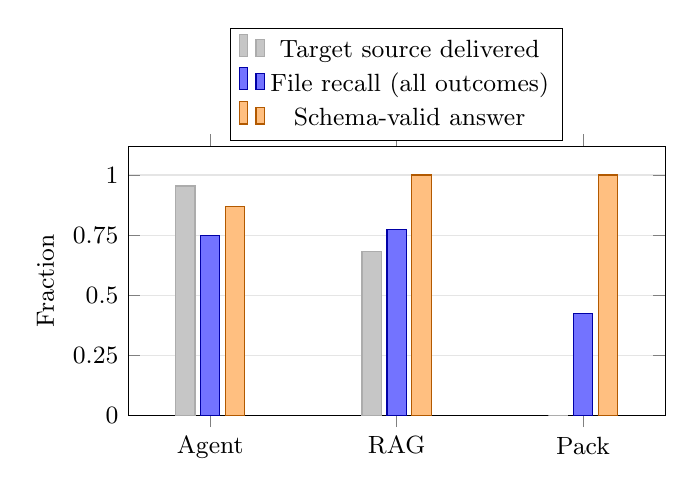
\begin{tikzpicture}
\begin{axis}[width=8.4cm,height=5.0cm,ybar,bar width=7pt,
      symbolic x coords={Agent,RAG,Pack},xtick=data,ymin=0,ymax=1.12,
      ylabel={Fraction},ytick={0,.25,.5,.75,1},
      tick label style={font=\small},label style={font=\small},
      ymajorgrids=true,grid style={gray!20},
      legend style={at={(.5,1.02)},anchor=south,legend columns=1,font=\small},
      enlarge x limits=.22]
      \addplot[fill=gray!45,draw=gray!65] coordinates {(Agent,0.954166666667) (RAG,0.681250000000) (Pack,0.000000000000)};\addlegendentry{Target source delivered}\addplot[fill=blue!55,draw=blue!65!black] coordinates {(Agent,0.747916666667) (RAG,0.772916666667) (Pack,0.422916666667)};\addlegendentry{File recall (all outcomes)}\addplot[fill=orange!50,draw=orange!70!black] coordinates {(Agent,0.870833333333) (RAG,1.000000000000) (Pack,1.000000000000)};\addlegendentry{Schema-valid answer}\end{axis}
\end{tikzpicture}\end{document}
